\documentclass[12pt]{article}
\usepackage[utf8]{inputenc}
\usepackage{tikz}
\usetikzlibrary{circuits.logic.US, positioning}
\usepackage{geometry}
\geometry{margin=1in}
\usepackage{amsmath}
\setlength{\parindent}{0pt}

\title{Cornell Notes: S-R Latch}
\date{02-07-2025}
\author{}

\begin{document}

\maketitle

\section*{Cues / Questions}
\begin{itemize}
    \item What is an S-R Latch?
    \item What are its inputs and outputs?
    \item How does it behave with different input combinations?
    \item What is the invalid state?
    \item What is the difference between NOR and NAND based latches?
    \item What are its applications?
\end{itemize}

\section*{Notes}

\textbf{Definition:} \\
The \textbf{S-R (Set-Reset) Latch} is a fundamental sequential circuit used to store 1-bit of data. It has two inputs: \textbf{Set (S)} and \textbf{Reset (R)}, and two outputs: \textbf{Q} and its complement \textbf{Q'}.

\vspace{1em}
\textbf{NOR-based S-R Latch (Active-High)}

\begin{center}
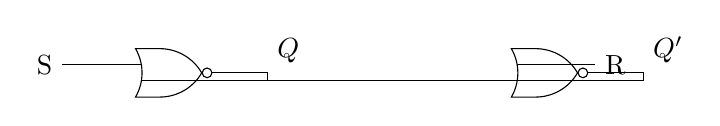
\begin{tikzpicture}[circuit logic US, logic gate inputs=nn, every node/.style={transform shape}, node distance=2cm]
    % Gates
    \node[nor gate, draw, rotate=0] (G1) {};
    \node[nor gate, draw, rotate=0, right=4cm of G1] (G2) {};

    % Feedback wires
    \draw (G1.output) -- ++(0.7,0) |- (G2.input 2);
    \draw (G2.output) -- ++(0.7,0) |- (G1.input 2);

    % Inputs
    \draw (G1.input 1) -- ++(-1,0) node[left] {S};
    \draw (G2.input 1) -- ++(1,0) node[right] {R};

    % Outputs
    \draw (G1.output) -- ++(0.7,0) node[above right] {$Q$};
    \draw (G2.output) -- ++(0.7,0) node[above right] {$Q'$};
\end{tikzpicture}
\end{center}

\vspace{1em}
\textbf{Truth Table (NOR-based S-R Latch):}

\begin{center}
\begin{tabular}{|c|c|c|c|}
\hline
S & R & Q (Next State) & Q' \\
\hline
0 & 0 & No Change      & Previous \\
0 & 1 & 0              & 1 \\
1 & 0 & 1              & 0 \\
1 & 1 & Invalid        & Invalid \\
\hline
\end{tabular}
\end{center}

\vspace{1.5em}
\textbf{NAND-based S-R Latch (Active-Low)}

\begin{center}
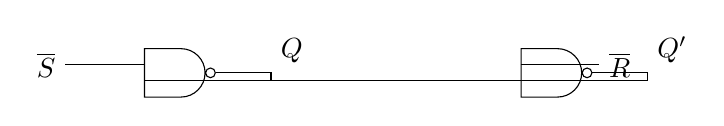
\begin{tikzpicture}[circuit logic US, logic gate inputs=nn, every node/.style={transform shape}, node distance=2cm]
    % Gates
    \node[nand gate, draw, rotate=0] (G1) {};
    \node[nand gate, draw, rotate=0, right=4cm of G1] (G2) {};

    % Feedback wires
    \draw (G1.output) -- ++(0.7,0) |- (G2.input 2);
    \draw (G2.output) -- ++(0.7,0) |- (G1.input 2);

    % Inputs
    \draw (G1.input 1) -- ++(-1,0) node[left] {$\overline{S}$};
    \draw (G2.input 1) -- ++(1,0) node[right] {$\overline{R}$};

    % Outputs
    \draw (G1.output) -- ++(0.7,0) node[above right] {$Q$};
    \draw (G2.output) -- ++(0.7,0) node[above right] {$Q'$};
\end{tikzpicture}
\end{center}

\vspace{1em}
\textbf{Truth Table (NAND-based S-R Latch):}

\begin{center}
\begin{tabular}{|c|c|c|c|}
\hline
$\overline{S}$ & $\overline{R}$ & Q & Q' \\
\hline
1 & 1 & No Change      & Previous \\
1 & 0 & 0              & 1 \\
0 & 1 & 1              & 0 \\
0 & 0 & Invalid        & Invalid \\
\hline
\end{tabular}
\end{center}

\vspace{1.5em}
\textbf{Applications:}
\begin{itemize}
    \item Single-bit memory storage
    \item Switch debouncing circuits
    \item Basic control circuits
    \item Building block for flip-flops (D, JK)
\end{itemize}

\section*{Summary}

The S-R Latch is a foundational digital storage device. It operates with either NOR (active-high) or NAND (active-low) logic gates and can hold a binary state. Care must be taken to avoid the invalid condition where both inputs are active simultaneously. It forms the basis for more complex sequential logic elements like flip-flops.

\end{document}
